\section{Supplementary Materials}

\begin{figure}[ht]
    \centering
    \begin{subfigure}{0.49\textwidth}
        \centering
        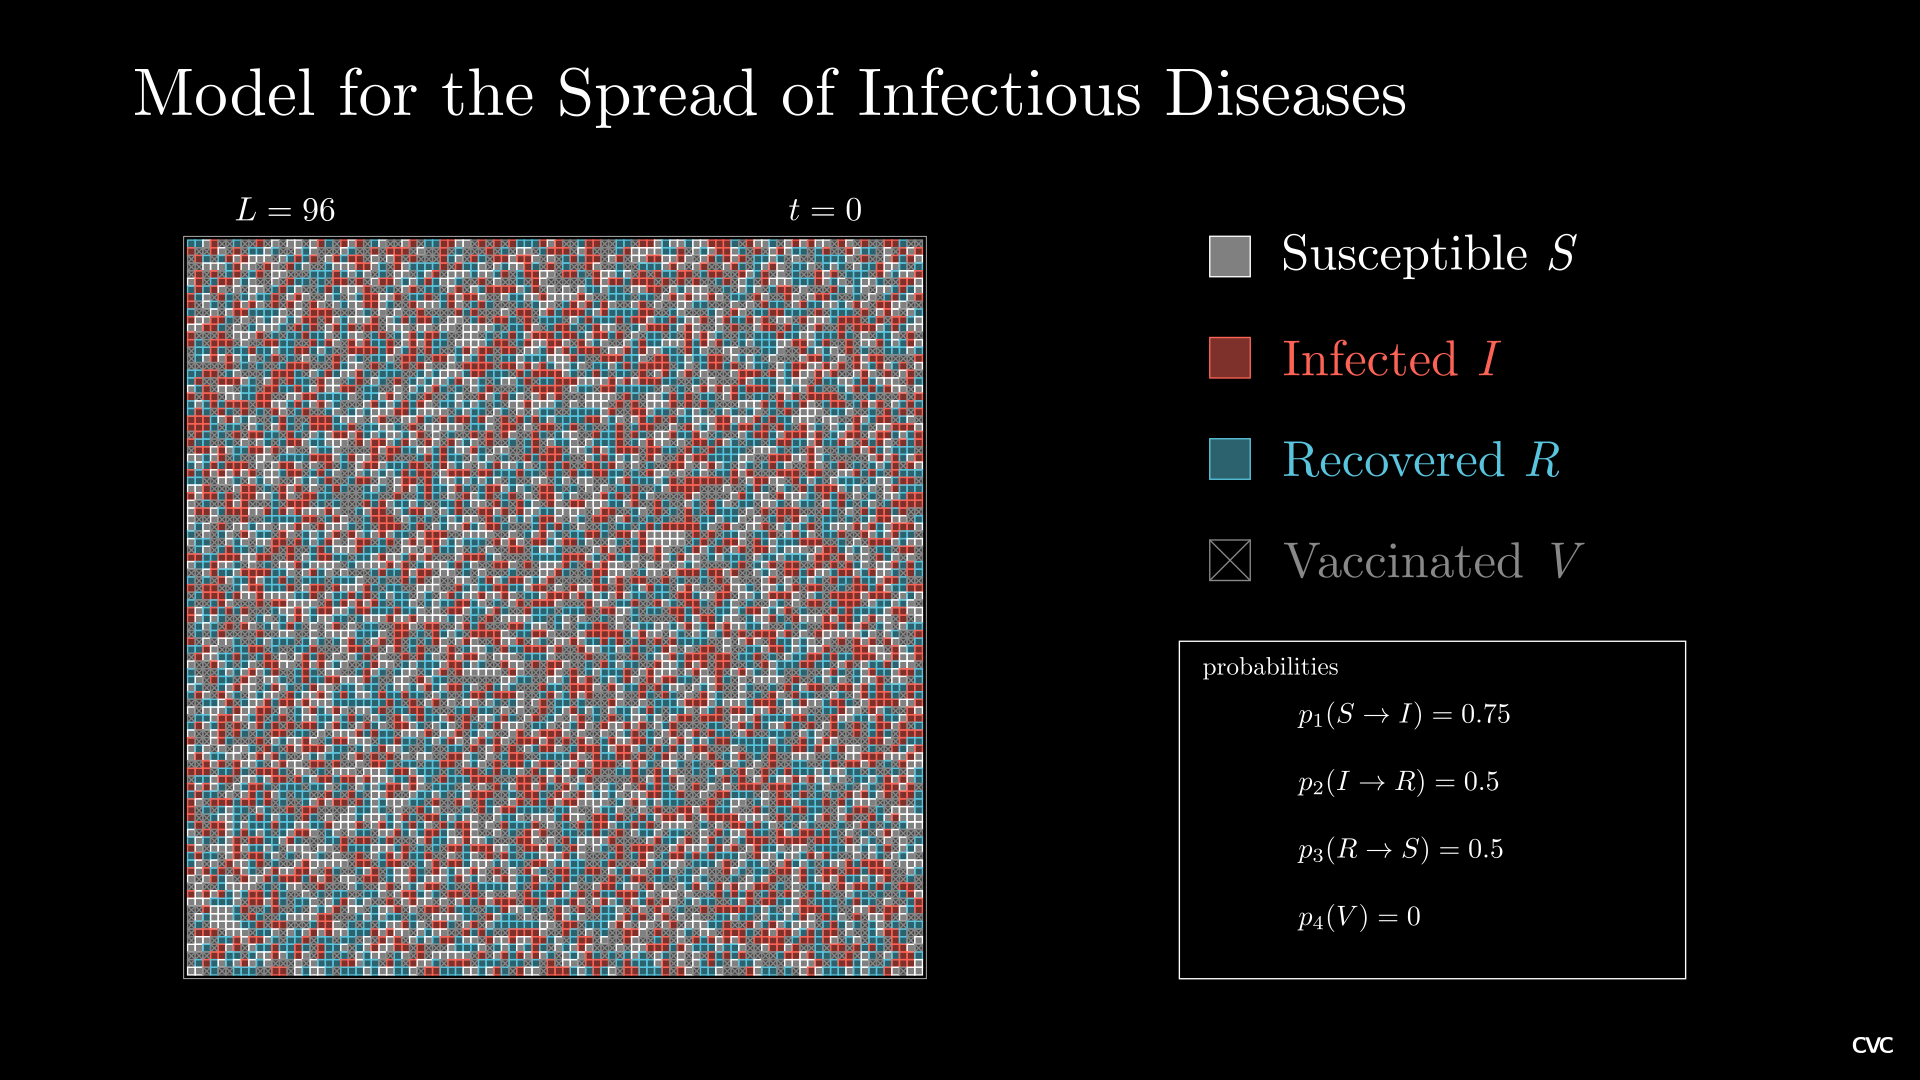
\includegraphics[width=1\textwidth]{images/soi_main_scene_75_50_50_25_init.png}
        \subcaption{\textbf(a) frame $t=0$}
    \end{subfigure}
    %\hspace{1cm}
    \begin{subfigure}{0.49\textwidth}
        \centering
        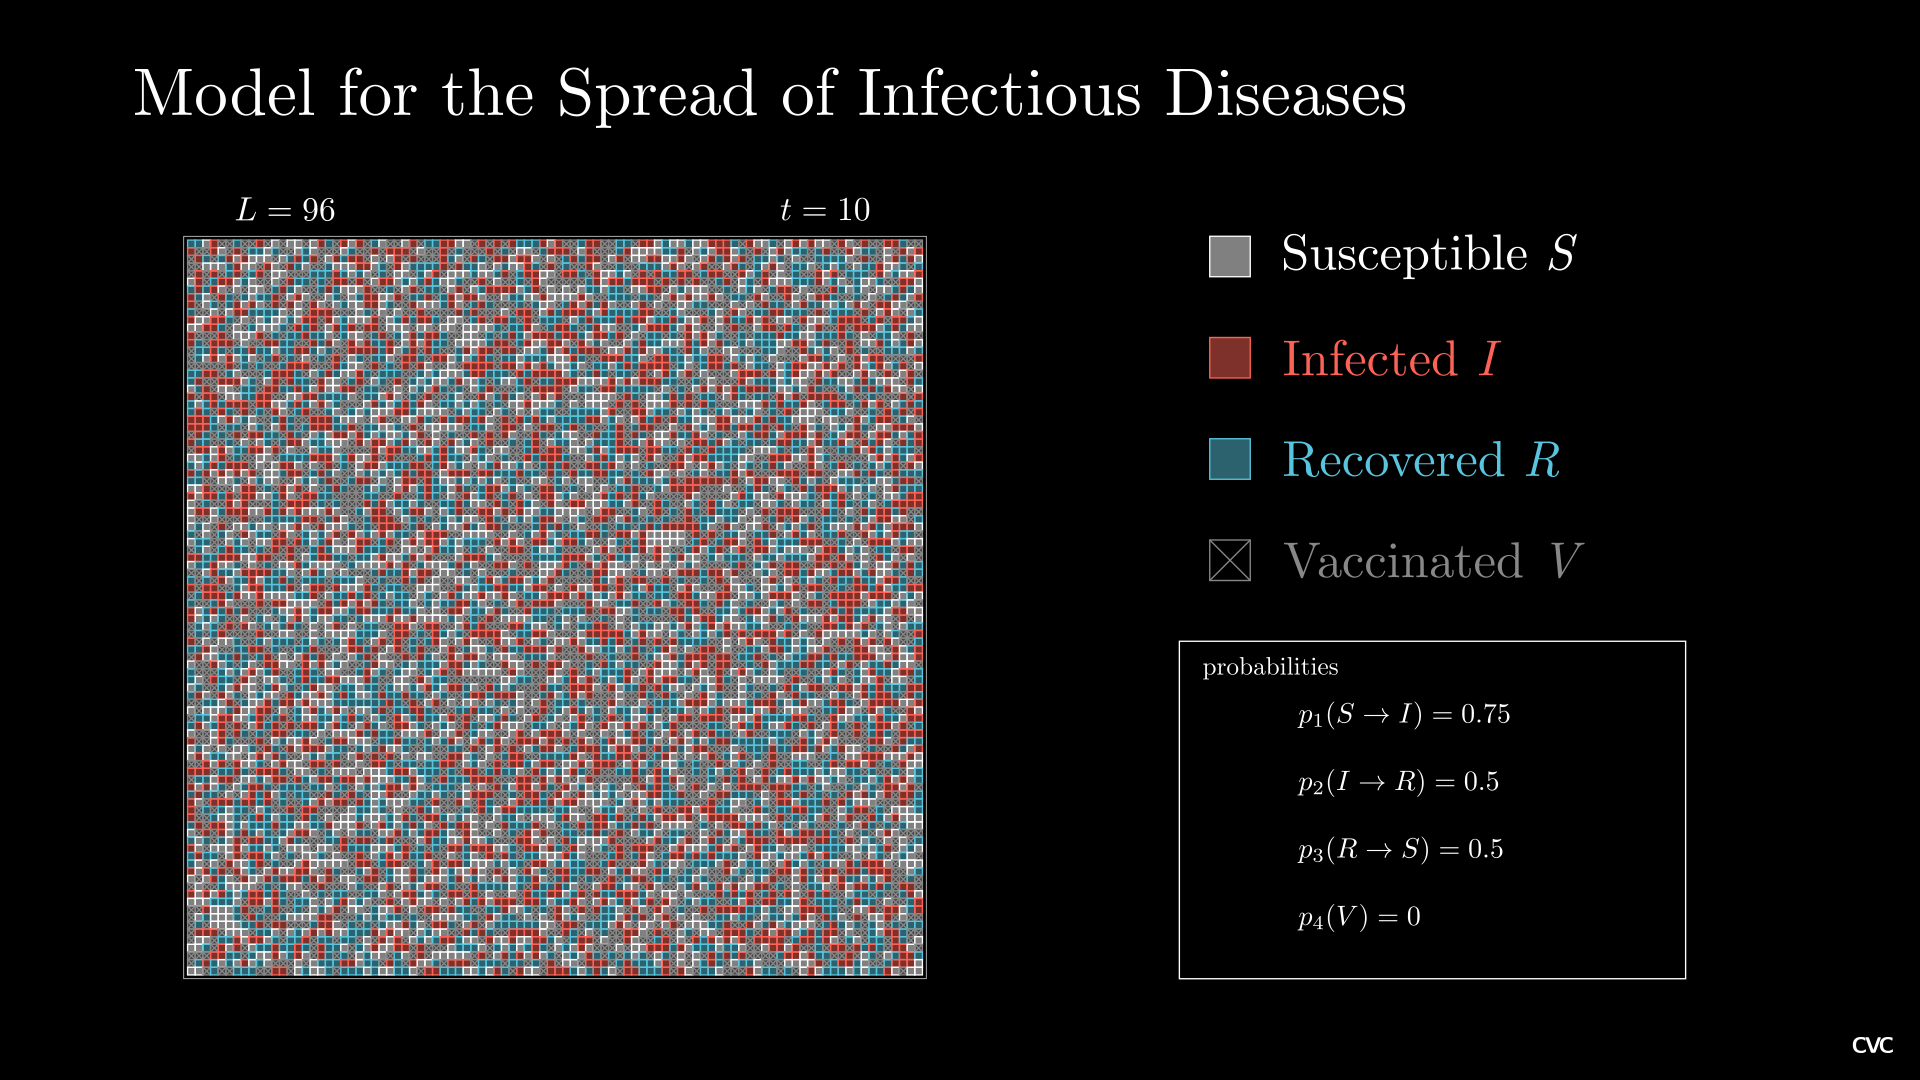
\includegraphics[width=1\textwidth]{images/soi_main_scene_75_50_50_25_t10.png}
         \subcaption{\textbf(b) frame $t=10$}
    \end{subfigure}
    \caption{Frames for simulation steps \textbf{(a)} $t=0$ and \textbf{(b)} $t=10$ of an animated simulation of the infectious disease model. The grid was initialized with a vaccination rate $p_4=0.25$
    and progressed with the turnover probabilities $p_1=0.75$, $p_2=p_3=0.5$}\label{fig:Animation_Inf_t}
\end{figure}